\documentclass[Bachelorarbeit.tex]{subfiles}
\begin{document}

\graphicspath{{./figures/implementation/}}	%specifying the folder for the figures

\chapter{Implementation}
\label{ch:implementation}

For this thesis a software was written to be able to investigate the behaviour and results of the different types of networks and get visual and numerical results to be embedded in this written text. In this chapter the implementation-details of the software are discussed.

\section{Requirements}
The author of this thesis had access to the software of \cite{Breuer2015} which was written in C++ therefore the question is why a new software had to be written and why not the original could be used. The reason for it was that the original software supported only a very narrow feature-set focusing only on the numerical results of a fully-connected network. Thus a complete redevelopment in Java was the option used. The following requirements were identified:

\begin{itemize}
\item Java based.
\item Comprehensive GUI functionality.
\item Emulate the functionality of \cite{Breuer2015} and its results.
\item Represent arbitrary networks in the simulation.
\item Step-through forward and backwards in a simulation-run.
\item Run replications of simulations.
\item Store results of replications to be opened again for later usage.
\item Command-line mode to run previously defined number of replications.
\end{itemize}

\paragraph{Java based}
The original software was written in C++ which offers very much power and highest speed if used correctly but comes with a very high responsibility regarding memory-management. Java offers a much more relaxed programming model regarding memory-management as it is garbage collected. This does not mean that the programmer can waste memory without giving thought to it but that not as many aufwand into it. debugging is easier.
The most compelling argument for Java are the vast libraries which are included in the JDK which are missing in standard C++. As complete GUI-functionality for the whole software is a requirement Java is the way to go. Although multi-purpose libraries like Boost and GUI-frameworks like Qt are available for C++ too, it takes quite some time to set them up correctly for the target platform one develops for which implies that in C++ the development would always have been for just one platform whereas Java runs on every platform - if not platform-dependent stuff was used - without recompilation. As one will see later in the "Command-line mode"-Feature this is a major requirement to make this feature practical. Thus the reasons for using Java were:

\begin{itemize}
\item Platform-independence which applies to 3rd party libraries too.
\item GUI-framework provided by JDK.
\item Relaxed memory-management which emphasises fast iterations and easy debugging.
\item Support for smooth XML-Serialization.
\item 3rd party libraries for network-modelling and -visualization.
\end{itemize}

\paragraph{GUI functionality}
All functionality should be accessible through a GUI where some features e.g. "Inspection" are only possible to use through a GUI.

\paragraph{Emulate \cite{Breuer2015} functionality}
Of course the whole software should be a super-set of the functionality of the one found in \cite{Breuer2015} so this was the point to start from.

\paragraph{Arbitrary networks}
It should be possible to restrict trading between the agents to arbitrary networks. As network-modelling and -visualization library JUNG is used.

\paragraph{Step-through simulation}
The software should support to go through a simulation-run step-by-step and storing all steps of the simulation to jump back and forth between steps.

\paragraph{Real-time visualisation and information}
The original C++ software didn't provide real-time information about the current wealth-distribution and market-dynamics and provided the user just with the numerical results in the end through the means of a command-line output. For better understanding of dynamics of both wealth and markets a real-time visualisation of both are necessary together with extensive information on the current state like the offering-book, agent-information, network-activity, history of matches and the current equilibrium. Also the real-time visualisation is necessary to provide this written part of the thesis with diagrams of various results and processes.

\paragraph{Replications}
Because the whole trading-process includes randomness the results are subject to noise thus replications are an absolute must-have feature to be able to give reliable results. Each replications is independent from all others thus it is a candidate for parallel programming to speed up the already very time-consuming process of running replications. According to the number of CPU-cores the software should spawn threads up to the number of cores and run replications in parallel thus speeding up by a considerable amount of time.

\paragraph{Store results}
When running a bunch of replications for a given set-up the results of it should be automatically stored as XML to be accessible for later inspection thus conserving state and eliminating the necessity to re-run time-consuming simulation-runs with a high number of replications.

\paragraph{Command-line mode}
As already described replications are required to be implemented for parallel processing where up to the number of CPU-cores replications can run in parallel. When running a vast number of replications one does not need to GUI-functionality and most probably the machine is so occupied by the heavy work-load that a fließender usage of GUI would be not possible any-more. Thus replications should be runnable through a separate command-line mode of the thesis-software which reads information from a XML-File in which one can specify multiple simulation set-ups for which replications should be run. The command-line mode iterates through all configurations and runs the required replications and writes the result out for a later inspection. Obviously the more CPU-cores the faster a simulation-run with e.g. 50 replications finishes. For this reason most of the final replication-runs were done on a 40-core machine of the FH Vorarlberg which runs on Linux on which the thesis-software could be run easily because of Java's platform-independence.

\section{Functionality}
In this section the functionality of the thesis-software is explained to get an understanding of the implemented features. All features are available through the GUI unless stated otherwise. For inspection, replications and experimenter an individual tab is available inside the main window so they can be used in parallel.

\subsection{Emulate \cite{Breuer2015} functionality}
Of course the starting point was to emulate the features of the \cite{Breuer2015} paper so all three markets were implemented together with "Bonds Pledgeability". In a first iteration the implementation was lacking the BP-feature which resulted in quite chaotic results which didn't come even close to the equilibrium shown in \cite{Breuer2015} which is a proof for the very importance of BP.
TODO: Noch unvollständig

\subsection{Inspection}
Inspection allows for a given simulation-configuration to step through the whole process match-by-match, keep track of the successful matches and the wealth-distribution of the agents at this time and to jump back to each successful match. Through an offer-book the state and current offerings of all agents at a given time of the simulation (including past successful matches) can be inspected and compared by opening multiple offer-book windows. Furthermore this feature provides the user with statistics of successful, failed and total matches and the current equilibrium. Very much attention was paid to the implementation of the real-time visualisation of the agents wealth-distribution and the market-activities as visualisation is of very importance for a successful inspection and interpretation of a dynamic process. To be able to compare the visual results of 2 different simulation-configurations there exist 2 "Inspection" tabs in the main window.

\subsection{Networks}
This functionality allows to model different kind of network-topologies as described in appendix \ref{app:topologies} "Topologies" to restrict trading only to this kind of neighbourhood. Obviously network-topologies are graphs and thus it would have been required to implement a graph-library but that was not implemented self but the graph-library JUNG was used as it supported all the required features like visualisation, neighbourhood- and path-queries.

\subsection{Replications}
To get robust results replications are used to reduce the influence of random noise. This feature allows to let run a specific simulation configuration for a given number of replications in parallel. The specific simulation-configuration serves as a template - especially the network-topology - and each replication does a clone of the network together with the agents to be able to run in parallel without the need of synchronization. It was tried to implement the network as a shared network between all replications but because the agents serve as nodes this was not feasible and would have required a very fundamental re-factoring of already existing functionality. Thus the higher requirements in memory and time for cloning was accepted for a more elegant solution.
When replications are processed running ones can be inspected and information can be queried using the GUI. It is possible to cancel one replication, cancel a whole task which reduces thread-load, inspect wealth-distribution, see the failed and successful matches and statistics of already finished replications. Whenever a replication is finished it is added to the pool of results and the median result is re-calculated and visualized and informations updated. When all replications have finished the results are written to a new XML-file in the results-folder of the software. This result-file can be opened using the experiments-feature which is described next. A simulation-configuration can be saved as a separate new experiment-file or added to an existing experiment-file - see next section for experiments.

\subsection{Experiments}
The experiments-feature allows to open experiment-files and result-files of replication- and experiment-runs. An experiment-file is just a collection of simulation-configurations to be run for a given number of replications. When an experiment-file is opened all simulation-configurations are displayed in a list an each of them can be opened as a new replication-tab which in turn can be run as explained in section "Replications". To be able to coneveniently run all simulation-configurations of an experiment-file without needing user-interaction a command-line feature was implemented. For this purpose the jar-file LeverageCycleCMD.jar was built. Start an experiment-run by using the following command:

\begin{center}
\textit{java -jar LeverageCycleCMD.jar PATH-TO-EXPERIMENT-FILE MAX-THREADS-OPTIONAL}
\end{center}

Note that the number of threads to use is optional and when omitted the number of CPU-cores found on the system is used. 

\medskip

Each replication-run of a given simulation-configuration in the experiment-file produces a result-file with the name provided in the configuration. These result-files are dubbed result-files of experiment-runs as previously stated but are the same as the result-file of a replication-run as discussed in the section "Replications"
When opening a result-file a new tab is added to the main-window and the statistics of the run together with equilibrium-statistics are displayed. Furthermore the wealth-distirbution and market-acitivities are visualized and it is possible to view the statistics of each individual replication. Furthermore the user can display the network-topology used for this simulation-configuration which is important as random networks are different when created new.


\section{Architecture}
In this section the basic architecture of the thesis-software is discussed. It is important to note that this thesis is a fat-client and has its major emphasis not on the software-development aspect but on the visual- and numerical results where the accompanying software is just a tool for the means to calculate theses required results. Thus the architecture is guided by a simple division of layers into front-end, controller and back-end. The front-end is responsible for input and output of the user through GUI or command-line. The controller-layer provides encapsulated chunks of functionality of the back-end to the front-end. It is necessary to abstract, encapsulate and combine the stateful nature of communication with the back-end into a separate layer instead of polluting the front-end with it and creating unnecessary dependencies. The back-end layer provides the functionality where the real work is done e.g. simulation is executed.
\medskip
Theoretically the dependencies are top-down where the front-end includes only controller-functionality, the controller includes only back-end functionality and the back-end has no dependencies to the preceding layers. In this thesis-software a more pragmatic approach was chosen so this dogma was not followed where over-engineering and over-complication would have resulted when sticking strictly to the separation of dependencies. Thus in very few cases the controller- and back-end layer include front-end layer functionality to create different types of network topologies in a more convenient way. Also the front-end accesses instances of pure back-end classes for graphical visualisation and information purposes. Despite the seemingly flawed architecture the development-process has proven to be very smooth and expansions and refactorings went quite smoothly and always resulted in a better and clearer structure with reduced code-smell which is always a sign for a good architecture.

\begin{figure}[H]
	\centering
  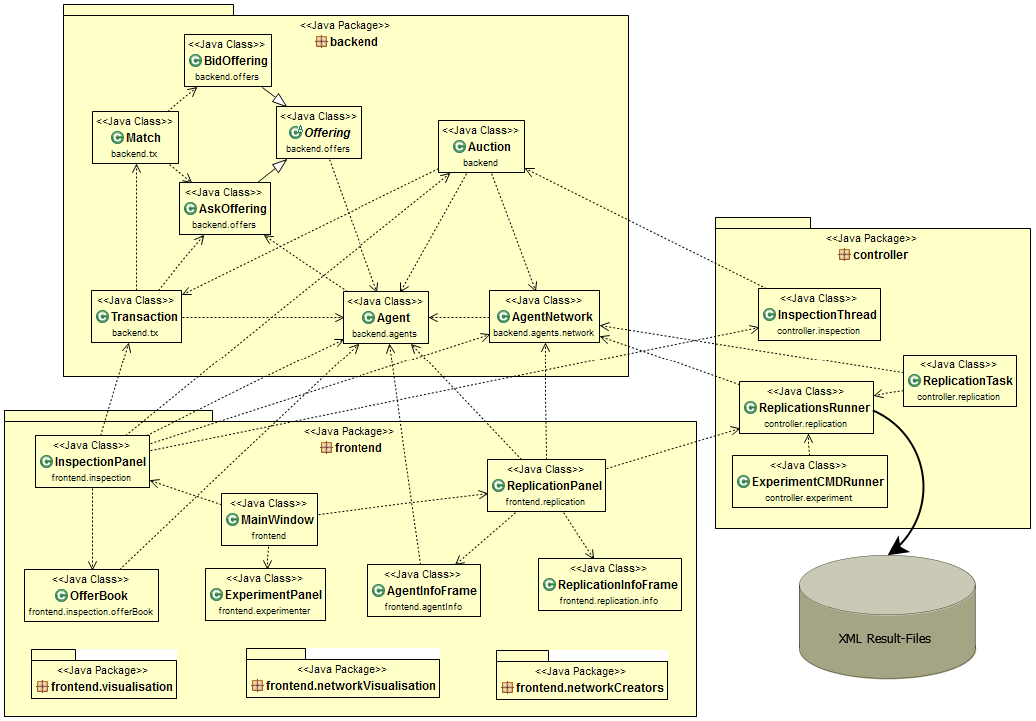
\includegraphics[width=1.0\textwidth, angle=0]{PACKAGE_DIAGRAM_MINIMAL.png}
	\caption{Package-diagram with most important classes and associations illustrating the architecture. (Note that the software contains many more classes and associations which are omitted for clarity reasons as this diagram should provide only a basic overview and would contain by far too much information if everything would have been included.)}
	\label{fig:PACKAGE_DIAGRAM_MINIMAL}
\end{figure}

\subsection{Frontend}
The front-end contains the GUI functionality through which the user interacts with the program and the real-time visualisation of wealth-distribution and market-activity. Because data like the offer-book, agent/replication/equilibrium-information and network-visualization is required in different contexts much emphasis was put on massive re-use of GUI components through the use of sub-classing and aggregation already provided by SWING. Thus many small components were implemented and aggregated together to create bigger chunks of logical functionality. In the package-diagram \ref{fig:PACKAGE_DIAGRAM_MINIMAL} only the most important panels are shown. Those provide the main entry-point for the user to the given functionality as indicated by their names.
TODO: noch aufzählung und beschreibung der wichtigsten panels (inspection/replication/experiments panel)

\subsection{Controller}
The controller package is rather slim and contains the steering functionality to drive inspections, replications and experiments. Inspections are driven by the class \textit{InspectionThread} which allows to advance the simulation step-by-step using the consumer-producer paradigm through lock and wait functionality provided by Java through the use of its monitors. The classes \textit{ReplicationsRunner} and \textit{ReplicationTask} encapsulate functionality to run a number of replications for a given simulation-configuration in parallel, calculating the current median for all important values on-line and writing results to xml-files. Experiments are executed from the command-line through the use of the class \textit{ExperimentCMDRunner} where it cycles through all simulation-configurations of a experiment-configuration and uses \textit{ReplicationsRunner} to execute it in parallel. 
TODO: anstatt in prosa auzuzählen: itemize oder klassen und beschreiben dort

\subsection{Backend}
The back-end contains the domain-specific functionality for the simulation. The important classes can be seen in the package-diagram \ref{fig:PACKAGE_DIAGRAM_MINIMAL} but for better clarity each one is introduced briefly.

\begin{itemize}
\item Auction - holds the state and operations for a single simulation-run. This class does the sweeping and clearing discussed in section "Simulation", determines whether trading is still possible or not and calculates current equilibrium.  allows to run a matching-round
\item Agent - encapsulates the functionality and state necessary for the agents in the simulation. See next section "Agents" for a more in-depth discussion.
\item AgentNetwork - holds the connections between the agents and provides functionality to query neighbourhood, paths and connections between agents and random and sequential in-order iterator over all agents.
\item Offering - encapsulates the data necessary for offerings where there are two subclasses \textit{BidOffering} and \textit{AskOffering} to differentiate between the two types of offerings. See the section "Markets" on details of offerings.
\item Match - provides the functionality to create a match out of given offers and returning an instance of \textit{Match} through a factory-method. The \textit{Match} instance holds the price, amount and the offers which have matched. See section "Sweeping and Matching" on more details.
\item Transaction - encapsulates functionality to search for a match within a given neighbourhood, is used by \textit{Auction} class to sweep through the agents and is returned after a matching-round and provides necessary information about whether it was successful or not.
\end{itemize}

\section{Agents}
Although agents are used in this software it is not an agent-based simulation in the classical way as these agents are zero-intelligence ones and have no states of behaviour. That is each agent makes bid- and ask-offers on all markets if the constraints allow it where the prices are selected from random ranges which improve the utility of the agent - that means it makes always offers which would result in a profit.

\medskip

Each agent is characterized by its state where the main variables are:

\begin{itemize}
\item Id - the unique id of the agent in the range of the natural numbers in the range of [1..number of agents].
\item Optimism-factor \textit{h} - defines how optimistic the agent is in the range of [0..1] where 0 is most pessimistic and 1 is most optimistic. The distribution of the optimism-factor among the agents is linearly ascending with the id and is defined through the following equation: \linebreak $\textit{optimism-factor} = \frac{id}{\textit{number of agents} + 1}$
\item Cash holdings - the current cash holdings of the agent.
\item Assets holdings - the current asset holdings of the agent not including the assets granted as securities for giving loans.
\item Loan given - the amount of loans bought from / granted to other agents. For a given amount of loans the equal amount of assets are granted as security to the buyer of the loan. Thus this variable increases the amount of assets the agent can trade with.
\item Loan taken - the amount of loans sold to other agents. For a given amount of loans the equal amount of assets the equal amount of assets are granted as security to the buyer of the loan. Thus this variable decreases the amount of assets the agent can trade with as this amount of loans needs to be kept as securities.
\end{itemize}

\medskip

There are three important derived variables which are calculated from the previous ones:

\begin{itemize}
\item Collateralized assets - is the amount of assets which are bound through collateral obligations because of taken bonds. \linebreak $\textit{collateralized assets} = max( 0, \textit{loans taken} - \textit{loans given} )$
\item Free assets - is the amount of assets which are unbound and act not as security and are owned completely by the agent. \linebreak $\textit{free assets} = \textit{Assets holding} - \textit{Collateralized assets}$
\item Loans - is the net number of loans and calculated through $\textit{loans} = \textit{loans given} - \textit{loans taken}$. Thus this value is positive if the agent has granted more loans to other agents than received and it is negative if the agent has received more loans from other agents than granted.
\end{itemize}

Note that all variables cannot go negative except loans.

\section{Markets}
In this section all markets and their implementations are described. Each market is completely characterised by the following points:

\begin{itemize}
\item Products - the products traded on the corresponding market.
\item Price-ranges - the price-ranges in which an agent places profit-making offers on the market.
\item Bid- and Ask-Offerings - define the pre-conditions for an agent to make offerings on the market and the amount and the prices generated during an offer. \medskip
Note that in case of bid-offerings the price of the profit-making offer is drawn randomly between the minimum price and the limit-price because when buying one wants to buy below the expected value to make a profit where in case of ask-offerings the price is drawn randomly between the limit-price and maximum price because when selling one wants to sell above the expected value to make a profit.
\item Match-Table - In case of a match between two agents the wealth-exchange is declared where the wealth is increased/decreased as indicated by the +/- signs.
\end{itemize}

\subsection{Asset/Cash}
\subsubsection{Products}
Free assets are traded against cash. The buyer gets a specific amount of free assets for a given amount of cash where the seller gives away the specific amount of free assets and gets the given amount of cash.

\subsubsection{Price-Range}

\paragraph{minimum}
The minimum value of one asset in cash is the down-value pD tomorrow as defined in chapter \ref{ch:leverageCycle} "The Leverage Cycle". This value is obviously a constant for all agents.

\begin{center}
$\textit{min asset-price} = \textit{pD}$
\end{center}
 
\paragraph{maximum}
The maximum value of one asset in cash is the up-value pU tomorrow as defined in chapter \ref{ch:leverageCycle} "The Leverage Cycle". This value is obviously a constant for all agents.

\begin{center}
$\textit{max asset-price} = \textit{pU}$
\end{center}

\paragraph{limit}
The limit-price of an asset in cash depends on the optimism-factor \textit{h} of the agent where the most optimistic agent assigns pU and the most pessimistic pD as the price. Thus applying linear interpolation one receives the following equation.

\begin{center}
$\textit{limit-price asset} = h * pU + ( 1.0 - h ) * pD$
\end{center}

\subsubsection{Bid-Offering}
As amount one TRADING-UNIT of assets is selected but if there is not enough cash left to buy one TRADING-UNIT of assets then no bid-offer is made.

\begin{table}[H]
	\centering
	\caption{Bid-Offering parameters of Asset/Cash market}
	\begin{tabular} { l c r }
		\hline
		Pre-Condition & $\textit{cash holdings} > \textit{price of TRADING-UNIT assets}$  \\
		Asset-Price & $\mathrm{random}(\textit{min asset-price}, \textit{limit-price asset})$ \\
		Asset-Amount & $\textit{TRADING-UNIT}$ \\
		\hline
	\end{tabular}
\end{table}

\subsubsection{Ask-Offering}
Ask offers are generated only when the agent has at least one TRADING-UNIT of free assets left. As amount one TRADING-UNIT of assets is selected - in the thesis-implementation 0.1 - but if there are fewer free assets left then no offer is made.

\begin{table}[H]
	\centering
	\caption{Ask-Offering parameters of Asset/Cash market}
	\begin{tabular} { l c r }
		\hline
		Pre-Condition & $\textit{free assets} > \textit{TRADING-UNIT}$  \\
		Asset-Price & $\mathrm{random}(\textit{limit-price of asset}, \textit{max asset-price})$ \\
		Asset-Amount & $\textit{TRADING-UNIT}$ \\
		\hline
	\end{tabular}
\end{table}


\subsubsection{Match}

\begin{table}[H]
	\centering
	\caption{Wealth-Exchange during a match on Asset/Cash market}
	\begin{tabular} { l c c }
		& Seller & Buyer \\
		\hline
		Assets holdings & - matching-amount & + matching-amount \\
		Cash holdings  & + matching-price & - matching-price \\
		\hline
	\end{tabular}
\end{table}

\subsection{Bond/Cash}
\subsubsection{Products}
Bonds are traded against cash. The buyer grants the seller a loan in buying a bond from the seller thus the buyer gets a given bond-amount from the seller and gives a given cash-amount to the seller. For a given amount of sold bonds the equal amount of assets need to be hold as securities.

\subsubsection{Price-Range}

\paragraph{minimum}
The minimum value of one bond in cash is the down-value pD tomorrow as defined in chapter \ref{ch:leverageCycle} "The Leverage Cycle". This value is obviously a constant for all agents.

\begin{center}
$\textit{min bond-price} = \textit{pD}$
\end{center}
 
\paragraph{maximum}
The maximum value of one bond in cash is the face-value V tomorrow as defined in chapter \ref{ch:leverageCycle} "The Leverage Cycle". This value is obviously a constant for all agents.

\begin{center}
$\textit{max bond-price} = \textit{facevalue V}$
\end{center}

\paragraph{limit}
The limit-price of a bond in cash depends on the optimism-factor \textit{h} of the agent where the most optimistic agent assigns \textit{facevalue V} and the most pessimistic \textit{pD} as the price. Thus applying linear interpolation one receives the following equation.

\begin{center}
$\textit{limit-price bond} = h * V + ( 1.0 - h ) * pD$
\end{center}

\subsubsection{Bid-Offering}
Bid offers are generated only when the agent has any cash holdings. As amount one TRADING-UNIT of bonds is selected but if there is not enough cash left to buy one TRADING-UNIT of bonds then the amount of bonds is selected which can be bought with the remaining cash holdings.

\begin{table}[H]
	\centering
	\caption{Bid-Offering parameters of Bond/Cash market}
	\begin{tabular} { l c r }
		\hline
		Pre-Condition & $\textit{cash holdings} > 0$  \\
		Bond-Price & $\mathrm{random}(\textit{min bond-price}, \textit{limit-price of bonds})$ \\
		Bond-Amount & $\min (\frac{\textit{cash holdings} }{ \textit{Bond-Price} }, \textit{TRADING-UNIT} )$ \\
		\hline
	\end{tabular}
\end{table}

\subsubsection{Ask-Offering}
Ask offers are generated only when the agent has any free assets because when selling the agent needs to reserve as many free assets as security as bonds sold. As amount one TRADING-UNIT of bonds is selected but if there are fewer free assets left then the remaining amount of free assets is selected.

\begin{table}[H]
	\centering
	\caption{Ask-Offering parameters of Bond/Cash market}
	\begin{tabular} { l c r }
		\hline
		Pre-Condition & $\textit{free assets} > 0$  \\
		Bond-Price & $\mathrm{random}(\textit{limit-price of bonds}, \textit{max bond-price})$ \\
		Bond-Amount & $\min ({\textit{free assets} }, \textit{TRADING-UNIT} )$ \\
		\hline
	\end{tabular}
\end{table}

\subsubsection{Match}

\begin{table}[H]
	\centering
	\caption{Wealth-Exchange during a match on Bond/Cash market}
	\begin{tabular} { l c c }
		& Seller & Buyer \\
		\hline
		Loan Given & N/A & + matching-amount \\
		Loans Taken & + matching-amount & N/A \\
		Cash holdings & + matching-price & - matching-price \\
		\hline
	\end{tabular}
\end{table}

\subsection{Asset/Bond}
\subsubsection{Products}
Assets are traded against bonds. The buyer gets a specific amount of free assets for a given amount of bonds where the seller gives away the specific amount of free assets and gets the given amount of bonds.

\subsubsection{Price-Range}

\paragraph{minimum}
The minimum value of one asset in bonds is defined as the ratio of the minimum asset-price in cash to the maximum bond-price in cash. This value is obviously a constant for all agents.

\begin{center}
$\textit{min asset/bond price} = \frac{\textit{minimum asset-price}}{\textit{maximum bond-price}} = \frac{pD}{V}$
\end{center}
 
\paragraph{maximum}
The maximum value of one asset in bonds is defined in the ratio of the maximum asset-price in cash to the minimum bond-price in cash.

\begin{center}
$\textit{max asset/bond price} = \frac{\textit{maximum asset-price}}{\textit{minimum bond-price}} = \frac{pU}{pD}$
\end{center}

\paragraph{limit}
The limit-price in bonds of an asset in bonds depends on the optimism-factor \textit{h} and is just the ratio of the limit-price of the asset to the limit-price of the loans.

\begin{center}
$\textit{limit-price asset/bond} = \frac{\textit{limit-price asset}}{\textit{limit-price bonds}}$
\end{center}

\subsubsection{Bid-Offering}
Bid offers are generated only when the agent is not negative on free assets after the trade. As amount one TRADING-UNIT of a assets is selected. To calculate the free assets after a match the following steps are performed:

\begin{enumerate}
\item Start with current free assets holdings.
\item Subtract current collateral obligations.
\item Subtract taken loans after trade.
\item Add assets bought through trade.
\end{enumerate}

\begin{table}[H]
	\centering
	\caption{Bid-Offering parameters of Asset/Bond market}
	\begin{tabular} { l c r }
		\hline
		Pre-Condition & $\textit{free assets} >= \textit{0 after trade}$  \\
		Asset/Bond-Price & $\mathrm{random}(\textit{min asset/bond price}, \textit{limit-price of asset/bond})$ \\
		Asset/Bond-Amount & $\textit{TRADING-UNIT}$ \\
		\hline
	\end{tabular}
\end{table}

\subsubsection{Ask-Offering}
Bid offers are generated only when the agent is not negative on free assets after the trade. As amount one TRADING-UNIT of bonds is selected. To calculate the free assets after a match the following steps are performed:

\begin{enumerate}
\item Start with current free assets holdings.
\item Subtract current collateral obligations.
\item Add given loans after trade.
\item Subtract assets sold through trade.
\end{enumerate}

\begin{table}[H]
	\centering
	\caption{Bid-Offering parameters of Asset/Bond market}
	\begin{tabular} { l c r }
		\hline
		Pre-Condition & $\textit{free assets} >= \textit{0 after trade}$  \\
		Asset/Bond-Price & $\mathrm{random}(\textit{limit-price of asset/bond}, \textit{max asset/bond price})$ \\
		Asset/Bond-Amount & $\textit{TRADING-UNIT}$ \\
		\hline
	\end{tabular}
\end{table}

\subsubsection{Match}

\begin{table}[H]
	\centering
	\caption{Wealth-Exchange during a match on Asset/Loan market}
	\begin{tabular} { l c c }
		& Seller & Buyer \\
		\hline
		Loan Given & + matching-amount & N/A \\
		Loans Taken & N/A & + matching-amount \\
		Asset holdings & - matching-price & + matching-price \\
		\hline
	\end{tabular}
\end{table}

\section{Simulation}
In this section a few details of the simulation-implementation are discussed as they are not so obvious but interesting and important enough to be mentioned.

\medskip

As noted above in the section "Markets" bonds and assets are always traded in chunks of TRADING-UNITS which is 0.1 in case of assets and 0.2 in case of bonds. Note that it is nothing unusual to scale the initial wealth-endowments to 1.0 and trade parts of them as in the end the absolute endowment does not matter but the distribution over the agents so a transformation to natural numbers would not gain anything. What is much more important is that the system conserves wealth: no wealth is lost and no wealth is created \textit{ex nihilo}. This is guaranteed by the equations and pre-conditions found in section "Markets". 

\subsection{Sweeping and Matching}
\label{sec:implementation_sweepingAndMatching}

\paragraph{Sweeping}
Sweeping is the process of generating a successful match by running through the agents and apply matching between their offers. Because offering-prices are created randomly in specific ranges it could happen that no offers match. To elevate this problem not only 1 but up to 500 sweeps are done when calculating the next successful match.

\begin{algorithm}
\caption{Sweeping Pseudocode}\label{euclid}
\begin{algorithmic}[1]
\State \textit{clear best offerings of all agents}
\While{ $sweeps < 500$ }
	\State \textit{clear global offerings of previous sweep}
	\State \textit{shuffle agents}
	\State \textit{generate offerings for all agents}
	\ForAll {shuffled agents}
		\State \textit{find match in neighbourhood}
		\If{ match found }
			\State \textit{execute match}
			\State \textbf{exit sweeping}
		\EndIf 
	\EndFor
	\If{ no trading possible }
	\State \textbf{exit sweeping}
	\EndIf
\EndWhile
\end{algorithmic}
\end{algorithm}

\paragraph{Matching}
Matching is the process of finding a match of a given agent in the sweeping-process with the offerings of its neighbourhood. Note that a match can only occur on one specific market between two agents thus satisfying only one buy- and one sell-offer.

\begin{algorithm}
\caption{Matching Pseudocode}\label{euclid}
\begin{algorithmic}[1]
\State \textit{get best offerings of neighbourhood}
\ForAll{neighbourhood offerings}
	\State \textit{randomly check sell or buy offerings first}
	\If{ $\textit{buy-price} \geq \textit{sell-price}$ }
		\State $m \gets \textbf{new Match}$
		\State $m.price = \frac{\textit{buy-price} + \textit{sell-price}}{2}$
		\State $m.amount = \min(\textit{buy-amount}, \textit{sell-amount})$
		\State $m.normPrice = m.price * m.amount$
		\State \textbf{exit matching}
	\EndIf
\EndFor
\end{algorithmic}
\end{algorithm}

\begin{algorithm}
\caption{Get Best Offerings of Neighbourhood Pseudocode}\label{euclid}
\begin{algorithmic}[1]
\State $\textit{bestOfferings} \gets \textit{null}$
\State $a \gets \textit{current agent}$
\ForAll{neighbours of a}
	\State $n \gets \textit{next neighbour of a}$
	\State $\textit{neighbourOfferings} \gets \textit{n.currentOfferings}$
	
	\ForAll{neighbourOfferings}
		\State $nO \gets \textit{next offering in neighbourOfferings}$
		
		\ForAll{bestOfferings}
			\State $bO \gets \textit{next offering in bestOfferings}$
		
			\If{nO.price dominates bO.price}
				\State $bO \gets nO$
			\EndIf
		\EndFor
	\EndFor
\EndFor
\end{algorithmic}
\end{algorithm}

Note that as defined in the double-auction theory - see chapter \ref{ch:theory} "Continous Double-Auction" - the agents meet at the half-way price. This guarantees that not more than the previously defined amount is traded which again conserves the wealth. Care must be taken when calculating the real price of the match as all offering prices are for 1.0 Unit of the traded good. Thus to obtain the real matching-price the previously calculated half-way price needs to be scaled by the matching-amount to obtain the price for the given matching-amount.
\medskip
Also note that if one match is found on any market then the sweeping and matching is terminated and a successful match is returned thus the agents can place offers on all markets although the sum of the offers would be infeasible because only one offer will be satisfied and the other ones are thrown away.

\section{Performance improvement}
\label{sec:implementation_performanceImprovement}

\subsection{Local and Global Offer-book}
It is easy to see that the calculation of the best neighbourhood can be quite costly the more neighbours an agent has. For of the ascending-connected topology this is not a big deal but in the case of the fully-connected topology the impact is serious. Because fully-connected is an important topology as it serves as a benchmark for the others an optimisation was implemented specially suited for this kind of topology: the introduction of a global offer-book. Instead of calculating the best offerings within the neighbourhood all offers are checked against each other in a global offering-list during the time of offering-creation. After all offers have been generated this list contains only the best sell and ask offerings for each market. The step of calculating the best neighbourhood can then be omitted in the case of fully-connectedness because it would be the same as the global best-offerings list thus saving a substantial amount of processing time.

\subsection{Matching probabilities}

\paragraph{General matching}
For a match to happen the buyer-price must be larger or equal the seller-price. Thus as shown in chapter \ref{ch:hypothesis} a price higher than the seller-price can only be placed by a buyer which has a strictly larger optimism-factor than the seller because only then their offering-ranges have a chance to cover each other partly. Thus matching in general works between a seller with lower optimism-factor and a buyer with higher optimism-factor. As noted in chapter \ref{ch:leverageCycle} "The Leverage Cycle" agents place offering-prices randomly in their ranges which are specified in this chapter in section "Markets" so matching is also subject to randomness.
\medskip
To investigate the matching-probabilities one must look at the coverage probabilities of the matching-ranges. The limit-price of bidders increase with rising optimism-factor and thus the width of the bidding-range decreases because bidders make their offers in the range of [limit-price..pU]. The situation is the inverse for askers as their limit-price increases too but the width of their asking-range increases because they place their offers in the range of [pD..limit-price]. Thus obviously the larger the difference in the optimism-factor between a seller and a buyer - again note that buyers optimism-factors are strictly larger than those of their corresponding sellers - the more likely a match will happen as both ranges increase and cover much more total distance thus increasing the probability that prices will be drawn which match.
\medskip
The following formulas derive the probabilities that an asker and a bider with a given limit-price will match on the Asset/Cash market. First the coverage-range is calculated by subtracting the limit-price of the asker from the one of the bidder as the one of the bidder must be larger. Then the probabilities of the asker and of the bider to fall into the range of the coverage-range is calculated. Finally the probability that both the asker and bider range will match is calculated by multiplying the previously calculated probabilities. Note that a division by 2 needs to be done because of symmetrical reasons because it does not matter where in the range the prices will meet but because the buy-price has to be larger or equal than the seller-price only the half-range is available.

\begin{center}
$\textit{coverage-range} = \textit{limit-price bidder} - \textit{limit-price asker}$
\end{center}

\begin{center}
$p(asker) = \frac{\textit{coverage-range}}{ pU - \textit{limit-price asker} }$
\end{center}

\begin{center}
$p(bider) = \frac{\textit{coverage-range}}{ \textit{limit-price bider} - pD }$
\end{center}

\begin{center}
$p(asker | bider) = \frac{p(asker) * p(bider)}{2}$
\end{center}

\paragraph{Matching in ascending-connectedness}
When considering the Ascending-Connected topology matching-probabilities become quite an issue as each agent has only 2 neighbours where the one with lower optimism-factor is the seller and the one with higher optimism-factor is the buyer. Thus compared to fully-connectedness where agents - depending on their optimism-factor - have multiple buyers and sellers the matching-probabilities are likely to be very low. To get a better understanding of the matching-probabilities in ascending-connectedness three diagrams visualizing them are shown below. Note that for clarity only 30 agents are considered on the Asset/Cash market.
\medskip
The following figure \ref{fig:MATCHING_PROBABILITIES_30_INDIVIDUAL} visualizes the probabilities of pairwise neighbours to fall into their coverage-range as calculated by the formulas given above.

\begin{figure}[H]
	\centering
  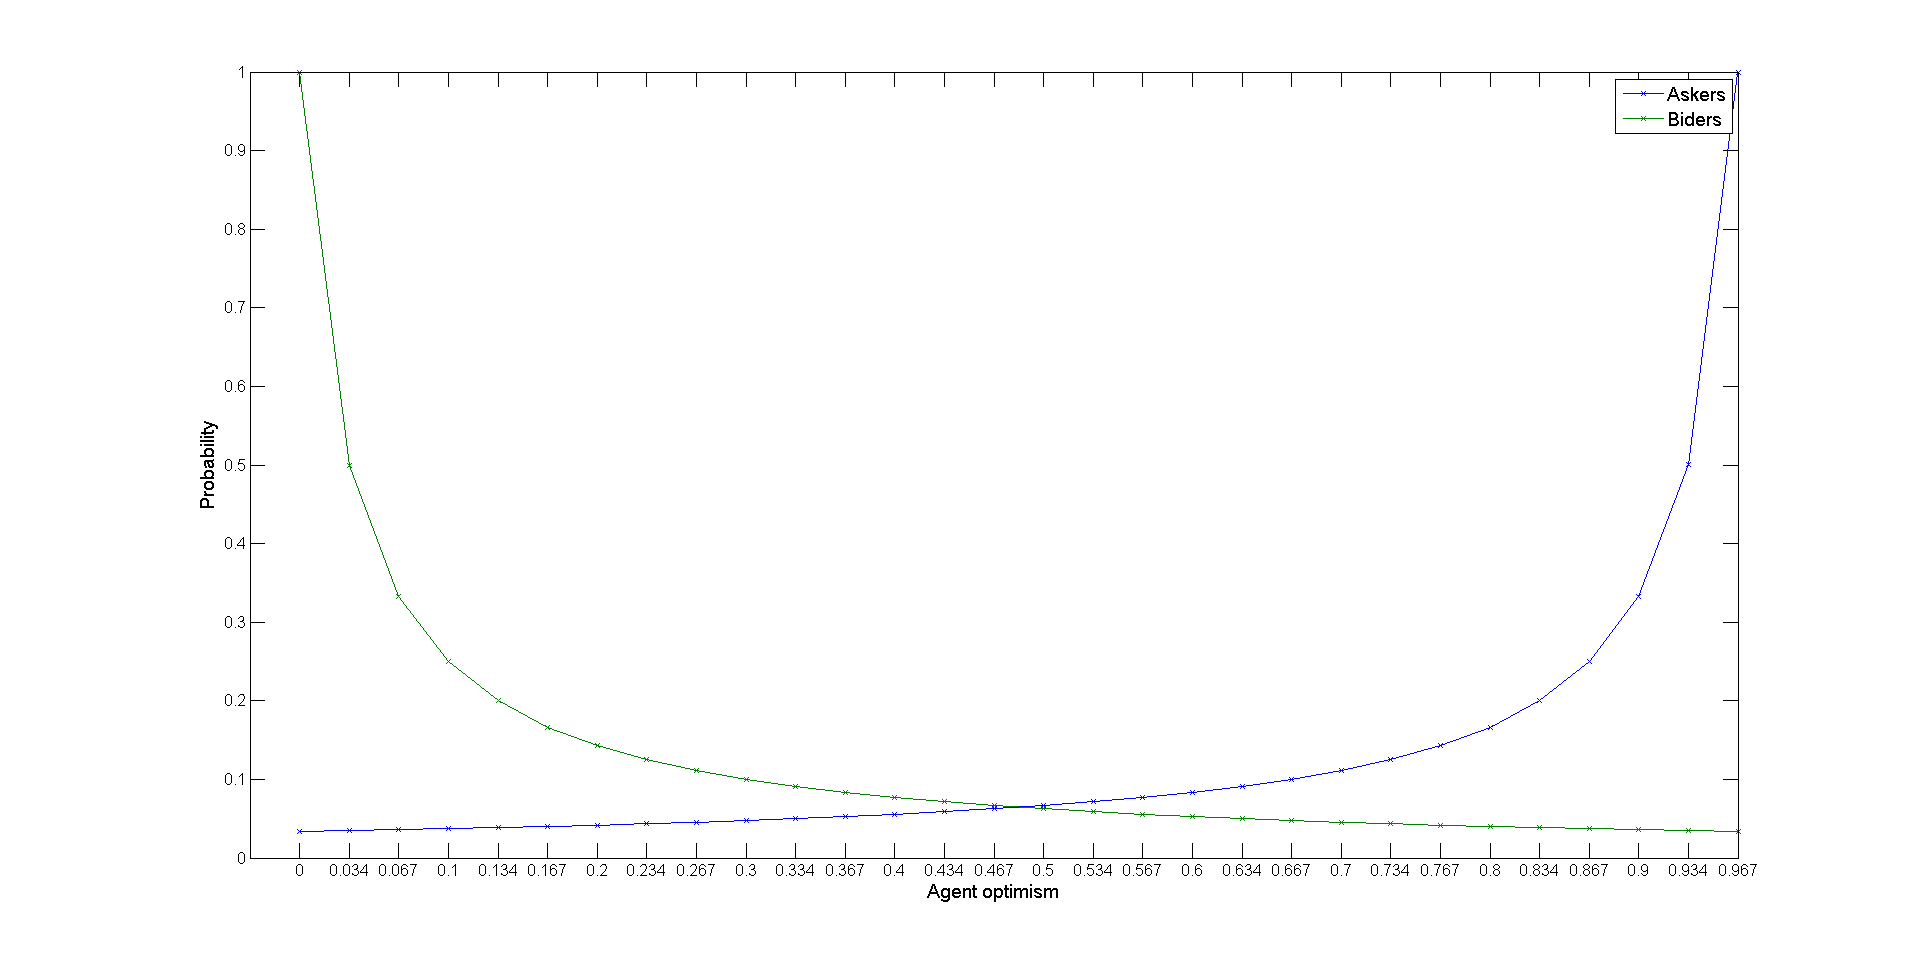
\includegraphics[width=1.0\textwidth, angle=0]{MATCHING_PROBABILITIES_30_INDIVIDUAL.png}
	\caption{Pairwise probabilities of falling into coverage-range of 30 agents in Ascending-Connected topology on Asset/Cash market}
	\label{fig:MATCHING_PROBABILITIES_30_INDIVIDUAL}
\end{figure}

The first bider with optimism-factor of 0.034 has a probability of 1.0 that the generated buy-prices fall into the range of its asker-neighbour with optimism-factor of 0. In turn the first asker with optimism-factor of 0 has a probability of 0.033 that its generated sell-prices fall into the range of its bid-neighbour with optimism-factor of 0.034. Thus the probabilities decrease for the bidders with increasing optimism-factor as their offering-range gets smaller and smaller where the probabilities increase for the askers with increasing optimism-factors as their offering-range gets wider and wider. This leads to the highest matching-probabilities at the edges and the lowest around the center.

The following figure \ref{fig:MATCHING_PROBABILITIES_30_COMBINED} visualizes the combined probabilities that asker and bider match their ranges.

\begin{figure}[H]
	\centering
  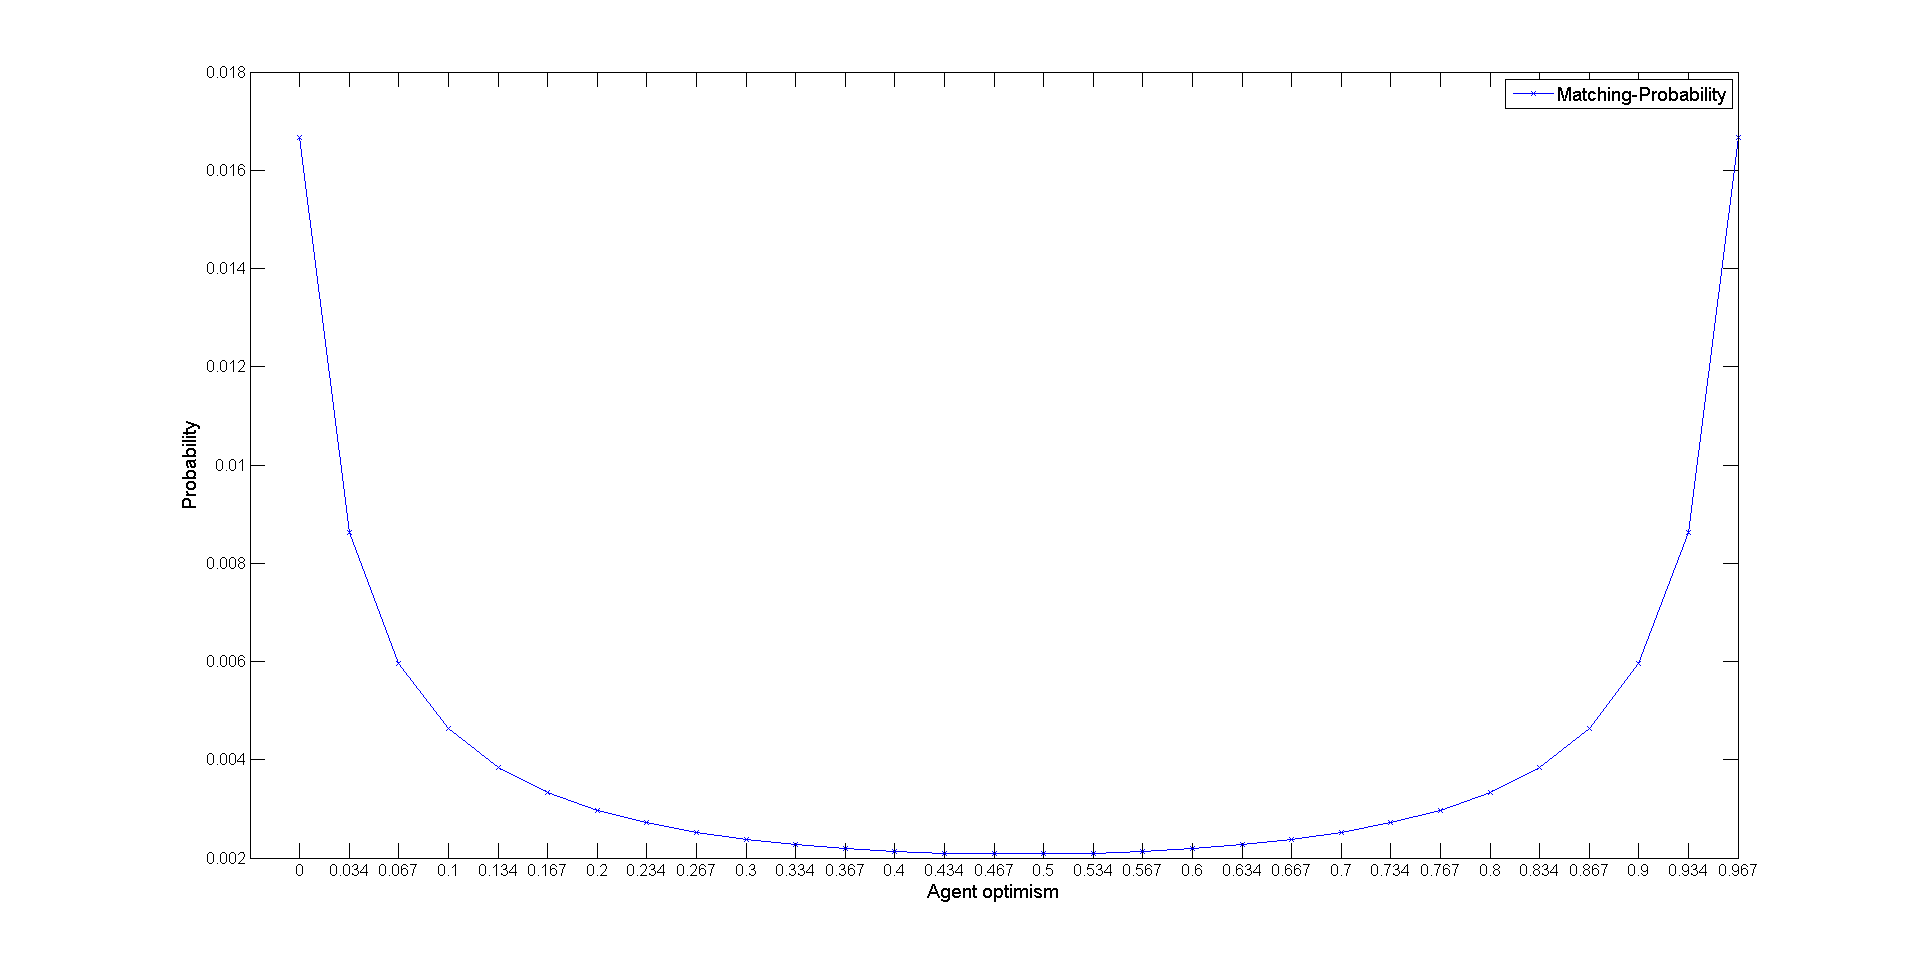
\includegraphics[width=1.0\textwidth, angle=0]{MATCHING_PROBABILITIES_30_COMBINED.png}
	\caption{Pairwise matching-probabilities of 30 Agents in Ascending-Connected topology on Asset/Cash market}
	\label{fig:MATCHING_PROBABILITIES_30_COMBINED}
\end{figure}

To see the influence of incresing number of agents the following figure \ref{fig:MATCHING_PROBABILITIES_50_COMBINED} visualizes the combined probabilities of 50 agents.

\begin{figure}[H]
	\centering
  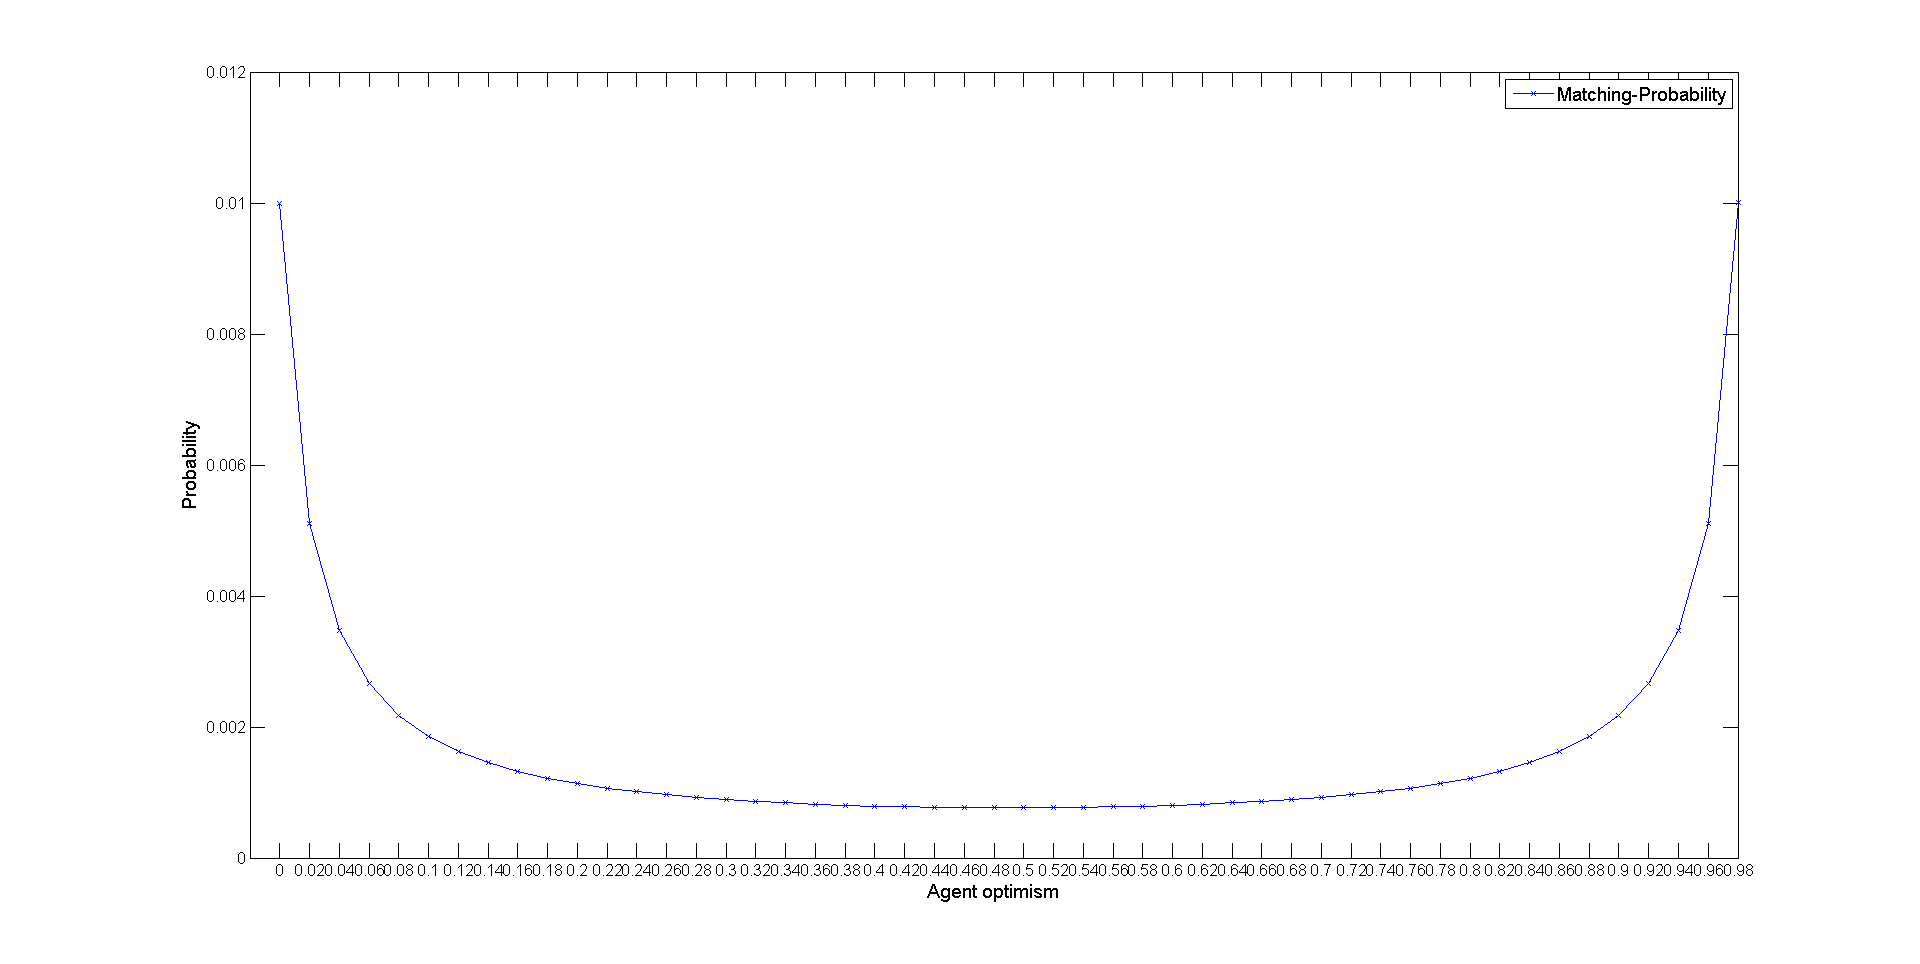
\includegraphics[width=1.0\textwidth, angle=0]{MATCHING_PROBABILITIES_50_COMBINED.png}
	\caption{Pairwise matching-probabilities of 50 Agents in Ascending-Connected topology on Asset/Cash market}
	\label{fig:MATCHING_PROBABILITIES_50_COMBINED}
\end{figure}

Looking at these diagrams one can derive the following facts about the matching-probabilities in Ascending-Connected topology:
\begin{enumerate}
\item Matching-probabilities are continuous and symmetric, are reduced towards the center of the optimism-scale and have their maximum at the very edges.
\item The more agents in the network the lower the matching-probabilities.
\end{enumerate}

The lower matching-probabilities result in longer simulation-runs and more inefficiencies towards the end where free assets are kept by optimists instead of traded as the matching-probabilities decrease so much that no more trading will occur. To elevate this problem one can adjust the matching-probabilities by transforming the price-ranges. It is of very importance that the shape of the matching-probabilities distribution must be exactly the same. Only the absolute values of the probabilities are increased where the edges are at the maximum of 1.0. This is mathematically quite involved and was not developed by myself but by Supervisor Mr. Vollbrecht. The formulas and explanations have been moved to appendix \ref{app:increasingMatchingProbability} "Increasing the matching-probabilities in Ascending-Connected topology"
\medskip
This variant is dubbed "Ascending-Connected topology with Importance Sampling". See chapter \ref{ch:results} "Results" for the performance and results of this variant.

\section{Calculating theoretical Equilibrium}
Theoretical equilibrium is known and specified through the equations given in section \ref{ch:leverageCycle} "Collateral Equilibrium" of chapter \ref{ch:leverageCycle} "The Leverage Cycle". This theoretical equilibrium is only applicable for an infinite number of agents whereas in the simulation a finite set of agents is used for which the theoretical equilibrium must be found too. For this purpose \cite{Breuer2015} developed an algorithm in MATLAB which searches the finite solution-space for the given equilibrium. This section gives a short overview of how the algorithm solves this task and is based on an existing document written by Martin Jandacka and the MATLAB code which both were available to the author of this thesis. Thus this section is only a simplified summary and the algorithm and the method behind it was not developed by the author of this thesis.

\medskip

For given asset prices q and bond-prices q each agent optimises its expected utility. As can be seen in the section "Markets" the utility-functions are linear which makes this optimization problem a linear one which can be solved by Linear Programming (LP). The only feasible vertices are:

\begin{itemize}
\item Cash only - hold by pessimists
\item Bonds only - hold by medianists
\item Assets financed by Bonds (no free assets) - hold by optimists 
\end{itemize}

Thus the two agents i1 and i2 are searched where i1 marks the end of the pessimists and i2 the beginning of the optimists. This is done by iterating through all possible combinations of i1 and i2 and checking if they generate equilibrium on the market or not. Thus time dependence is $O(n^2)$ where n is the amount of agents. 

\end{document}
